\subsection{Time Delays}

\begin{wrapfigure}{R}{0.4\textwidth}
\centering
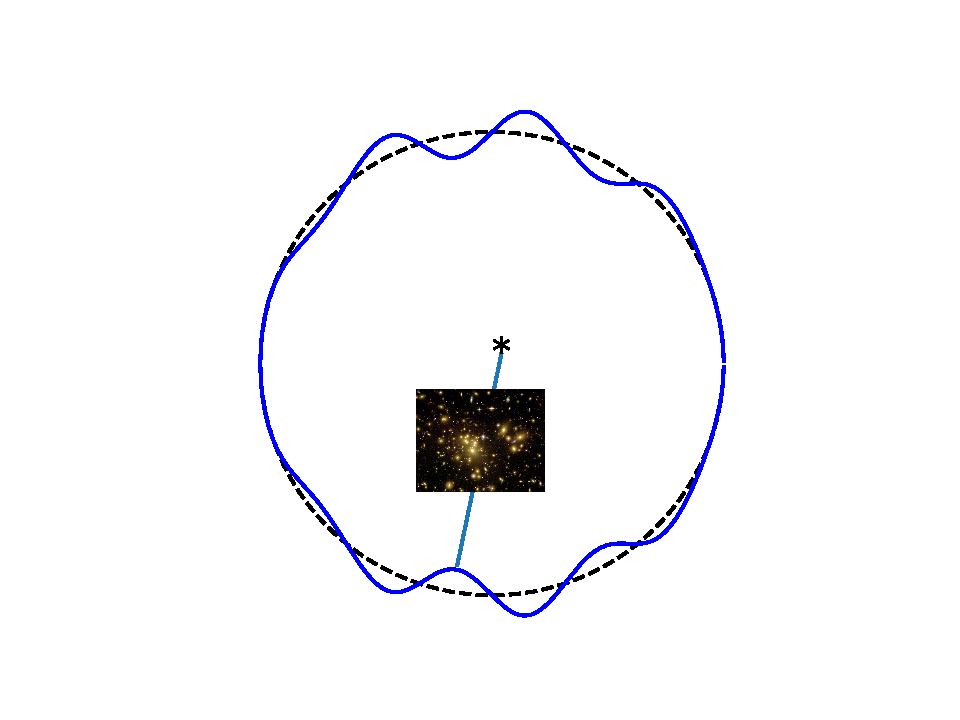
\includegraphics[width=0.4\textwidth]{td.pdf}
\caption{\footnotesize \label{fig:td}Schematic of the impact of time
  delays on the last scattering surface with us at the center. Dashed
  line denotes the assumed spherical last scattering surface, while
  blue solid curve denotes the more realistic corrugated surface due
  to time delays. Rays that pass through over-dense regions (as
  depicted in the figure) are slowed down; since all photons were
  released from the electrons at the same time, these ``slower''
  photons travel shorter distances and therefore originated from
  closer distances than average.}
\end{wrapfigure}

Photons that comprise the CMB experience time delays or advances depending on the integrated potential through which they travel, as depicted in Fig.~\rf{td}. Since photons do not decouple instantaneously from the electron-proton plasma, the surface of last scattering is often said to have a finite width; however, the directional-dependent change in the distance to last scattering is independent of its finite width and is also different than the angular deflections that have been captured by recent experiments. 

The integrated potential that determines the time delays differs from the one that cause the deflections, so if we can measure time delays, we will have measured a new cosmic field. As an estimate of how viable this is, we follow the formalism of \citet{okamoto} and to obtain estimators that are quadratic in the CMB fields (temperature and two components of polarization). As an example the relevant estimator quadratic in temperature is
\be
\hat d_{LM} = B_{L} \sum_{l_1m_1}\sum_{l_2m_2}%\nonumber \\
 (-1)^M  \bigl(\begin{smallmatrix} l_1 & l_2 & L \\ m_1 & m_2 & -M  \end{smallmatrix}\bigr) h_{l_1l_2}(L)  \tob_{l_1m_1} \tob_{l_2m_2}\eql{tdest}
 \ee
 where the sum is over two angular momenta that can combine to form $LM$ and $h$ is a coefficient that depends on the {\it radial derivative} of the CMB power spectrum with respect to the distance to the last scattering surface: $\partial C_l/\partial \ln(D_*)$. This spectrum is depicted in Fig.~\rf{TT1}. 

\begin{wrapfigure}{R}{0.4\textwidth}
\centering
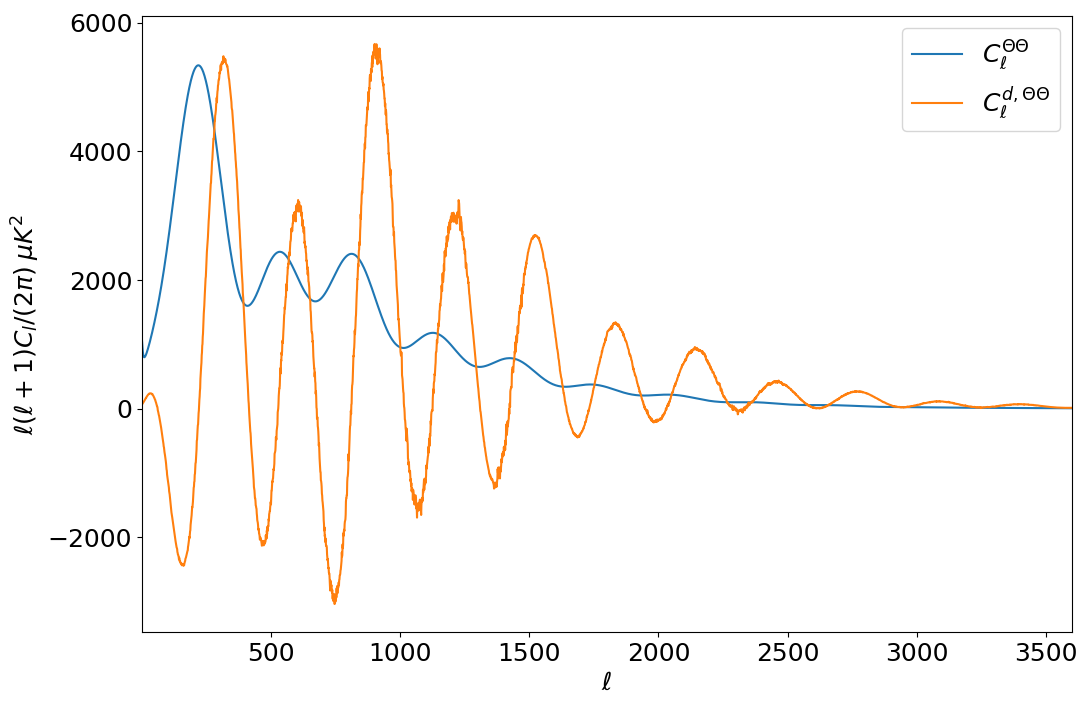
\includegraphics[width=0.4\textwidth]{TT1}
\caption{\footnotesize \label{fig:TT1} The standard CMB temperature
  power spectrum $C_l^{\Theta\Theta}$ compared to the one that is used
  in the estimator to extract time delays: $C^{d,\Theta\Theta}\equiv
  \partial C_l/\partial \ln(D_*)$.}
\end{wrapfigure} 

 The estimator in \ec{tdest} has an expectation value equal to the fractional difference in distance along the line of sight (actually the coefficients of that fractional distance field decomposed into spherical harmonics). Similarly, we can form estimators for combinations of the temperature and the two polarization fields and combine all estimators to estimate the signal to noise. Preliminary estimates point to the possibility of detection, but only with next generation surveys. We propose to develop these estimators to obtain reliable projections accounting for systematics. These projections can help inform the design capabilities of a survey such as CMB-S4. As described below, we also will work on the possibility of detecting time delays of the CMB behind galaxy clusters; i.e., in cross-correlation. Another possibility is to estimate not the power spectrum of the time delay field but rather the cross-spectrum of the deflection field (which has a larger amplitude) with the time delay field. In short, time delays offer exciting opportunities to open up new horizons in CMB analysis.
